% !TEX root = ../main.tex
%
\section{Introduction}
\label{sec:introduction}

Research on conversational moderation/facilitation techniques is crucial for adapting to ever-changing and demanding online environments. Relevant work traditionally focused on isolating and removing content \cite{seering_self_moderation, cresci_pesonalized_interventions}, whereas the current social media environment demands moderation systems to adequately explain their actions and prevent problematic behaviors before they surface \cite{cho-etal-2024-language, seering_self_moderation, cresci_pesonalized_interventions, make_reddit_great}.  Facilitation mechanisms are also needed to handle community deliberation and group decision-making \cite{kim_et_al_chatbot, seering_self_moderation}. Note that “content moderation” usually involves flagging and removing content, as opposed to “conversational moderation”, which is studied in this paper. The terms “facilitation” and “conversational moderation” are otherwise equivalent \cite{argyle2023, korre2025evaluation, falk-etal-2021-predicting} and we treat them as synonyms in this paper.

\begin{figure}[t]
	\centering
	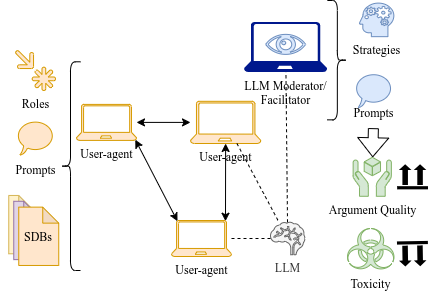
\includegraphics[width=\columnwidth]{research_goal.png}
	\caption{\ac{LLM} user-agents with distinct \acp{SDB} participate in a discussion, while the \ac{LLM} moderator monitors and attempts to improve the quality of the discussion. We need to design prompts and configurations for both types of \ac{LLM} agents.}
	\label{fig::goals}
\end{figure}

A major challenge in connecting facilitation research to real-world needs is the substantial costs required both in researching and moderating discussions, due to human participation \cite{rossi_2024}. Many social media platforms overcome this by outsourcing moderation to volunteers or their own users \cite{Matias2019TheCL, schaffner_community_guidelines}, while others support only conventional content moderation using traditional \ac{ML} models, which are not enough in practice \cite{horta_automated_moderation, schaffner_community_guidelines}. \acfp{LLM} have been hypothesized to be capable of facilitation tasks, which often require actively participating in the discussions, instead of passively flagging or removing content \cite{small-polis-llm, korre2025evaluation}. 

While studies exist for simulating user interactions in social media \cite{park_simulacra, mou_2024, tornberg_2023, y_social, balog_2024}, and for using \ac{LLM} facilitators \cite{kim_et_al_chatbot, cho-etal-2024-language}, none so far have combined the two approaches. We posit that synthetic simulations can be a cheap and fast way to develop and test preliminary experiments with \ac{LLM} facilitators, initial versions of which may be unstable or unpredictable \cite{atil_2025, rossi_2024}, before testing them with human participants. Our work thus asks the following two questions: (1) Can we produce high-quality synthetic discussions, involving alternative facilitation strategies, by crafting an appropriate environment for simulations? (2) Can we boost the effectiveness of \ac{LLM} facilitators (in synthetic discussions) using prompts aligned with facilitation strategies proposed in modern Social Science research?

We propose a simple and generalizable methodology (\S\ref{sec:methodology}) using \ac{LLM}-driven synthetic experiments for online facilitation research, enabling fast and inexpensive model “debugging” and parameter testing (e.g., finding \ac{LLM} facilitator instructions) without human involvement (Fig.~\ref{fig::goals}). An ablation study (\S\ref{ssec:results:ablation}) demonstrates that each component of our methodology qualitatively contributes to generating high-quality data. We examine four \ac{LLM} facilitation strategies based on current Social Science facilitation research---including a novel strategy inspired by \ac{RL}---(\S\ref{sec:experimental}) and compare them with two baselines (no facilitation, \acp{LLM} with simplistic prompts).

We find that: (1) the presence of \ac{LLM} facilitators has a positive and statistically significant influence on the quality of synthetic discussions, (2) facilitation strategies inspired by Social Science research often do not manage to outperform simpler baselines (\S\ref{ssec:results:main}).
Furthermore, we release \syndisco, an open-source Python framework for generating and evaluating synthetic discussions, alongside \vmd\datasetlink a large, publicly available dataset comprising automatically evaluated synthetic discussions (\S\ref{sec:data-soft}). 
We use open-source \acp{LLM} and include all relevant configurations in order to make our study as reproducible as possible (see \S\ref{ssec:appendix:annotation}, \S\ref{ssec:appendix:prompts}).